\documentclass[12pt]{article}

\usepackage{amsmath}
\usepackage{amssymb}
\usepackage{graphicx}
\usepackage[outdir=./]{epstopdf}
\usepackage{setspace}
\usepackage{geometry}
\usepackage{booktabs}
\usepackage{hyperref}
\usepackage{xurl}
\usepackage{float}

\geometry{margin=1in}
\setstretch{1.2}

\title{The Geometry of Governance: \\ A Topological Perspective on Institutional Manifolds}

\author{
Adriel I. Santoso \\
Department of Mechanical and Aerospace Engineering \\
Tohoku University
}

\date{\today}

\begin{document}

\maketitle

\begin{abstract}
While comparative political science often relies on discrete regime typologies, this paper explores the utility of modeling state architecture as a continuous, low-dimensional manifold. Grounded in the classic political theories of Marshall and Dahl, we construct an \textit{Institutional Triad} representing Order, Liberty, and Equality. Using cross-national data ($N=66$) and manifold learning techniques (PCA and UMAP), we map governance coordinates via institutional \textit{Magnitude} (mean capacity) and \textit{Imbalance} (structural skew). 

The analysis identifies a structural ``funnel'' pattern in the distribution of states, suggesting an empirical boundary constraint on development: while low-capacity states exhibit high structural variance, achieving the highest tiers of magnitude requires dimensional balance. However, multivariate OLS regressions find evidence for an ``Imbalance Premium'': controlling for magnitude, institutional imbalance positively associates with human development (HDI) and economic prosperity. We propose the \textit{Developmental Vanguard} hypothesis, suggesting that asymmetrical institutional growth may serve as a functional catalyst for escaping middle-income stagnation. These findings offer a topological perspective that complements existing categorical models and suggests new avenues for analyzing the geometry of political development.
\end{abstract}

\section{Introduction}

Comparative political science has long debated the relationship between state capacity, democratic freedoms, and economic justice. However, these debates frequently rely on discrete categorical models—e.g., classifying a state as an ``electoral autocracy'' or ``consolidated democracy'' (Bäck \& Hadenius, 2008). While heuristically useful, these categories may fail to capture the continuous, topological trade-offs states make when allocating power and resources.

Concurrently, systems theory and developmental models suggest that complex institutions do not evolve via discrete leaps, but through the continuous integration of specialized dimensions (Bertalanffy, 1968; Luhmann, 1995). If state institutions represent an integrated cognitive and organizational system, their development must be subject to structural and mathematical constraints.

This paper bridges formal systems theory and empirical political science by proposing a geometric framework for state architecture. We ask: Does state governance form discrete clusters, or a continuous manifold? What mathematical constraints govern how states prioritize competing institutional goals? Finally, how does the geometry of a state's institutional profile independently correlate with human prosperity?

\section{Theoretical Context}

This paper integrates formal theories of system complexity with the comparative political economy of institutions.

\subsection{Institutions and State Capacity}
Political and economic theory focus on the structure and function of institutions as the rules that organize social interaction (North, 1990). A central concept in this literature is \textit{state capacity}, defined as the institutional ability of political systems to implement decisions and coordinate action (Hanson \& Sigman, 2021). Analyses of state development emphasize the role of administrative organization, resource extraction, and institutional coherence in maintaining order (Fukuyama, 2011; Acemoglu \& Robinson, 2012). However, these approaches often analytically separate or contrast capacity and liberty rather than treating them as dimensions within a shared geometric space.

\subsection{Systems Theory and Development}
Systems-oriented perspectives analyze large-scale structures by focusing on system-level processes that operate independently of individual actors (Bertalanffy, 1968). Developmental frameworks emphasize that higher-order stability requires the progressive coordination of multiple systemic dimensions (Simon, 1962). Applying these insights to macro-politics suggests that the stability and prosperity of a nation rely not just on the absolute strength of its institutions, but on their mathematical balance and integration.

\subsection{Geometric and Unbalanced Perspectives on Governance}
A limited but emerging set of approaches employs geometric heuristics to conceptualize political phenomena. Blind (2014) uses concentric circles, triangles, and cubes to synthesize concepts such as transparency, accountability, and democratization, demonstrating the analytical utility of spatial metaphors. While Blind’s work remains largely metaphorical, the present paper extends this intuition by formalizing state architecture as a continuous manifold with axiomatic properties.

More directly, Acemoglu and Robinson (2019) propose a tripartite framework of state--society relations---absent leviathan, despotic leviathan, and shackled leviathan---arguing that liberty requires a balance between state power and societal mobilization. Their concept of the “narrow corridor” echoes the funnel constraint we formalize in Hypothesis 2. Meanwhile, a growing literature examines the effects of \textit{unbalanced} institutional development. Liu and Li (2019) find that, in emerging economies, institutional asymmetry can benefit firms by enabling strategic flexibility. We explore whether this micro-level logic of strategic flexibility extends to macro-level institutional development, yielding our ``Imbalance Premium'' in Hypothesis 4.

\subsection{The Institutional Triad: Foundations and Parsimony}

The selection of Order ($O$), Liberty ($L$), and Equality ($E$) synthesizes foundational theories of political development into a parsimonious geometric space. \textbf{Order} provides the requisite administrative capacity and security (Hobbes, 1651; Huntington, 1968). The remaining axes formalize Dahl’s (1971) classic dimensions of polyarchy: \textbf{Liberty} represents the degree of public contestation and negative constraints on state authority (Berlin, 1958; Acemoglu \& Robinson, 2019), while \textbf{Equality} captures the breadth of systemic participation and resource distribution (Rawls, 1971; Sen, 1999). 

While Marshall (1950) historically modeled the expansion of these rights—civil, political, and social—as sequential phases, our framework treats them as hierarchically concurrent. In this view, each emergent stage does not replace the previous one but integrates into a whole, expanding the manifold's dimensionality. The theoretical justification for this concurrency lies in the complexity of modern governance (Luhmann, 1995). A state does not cease to require foundational Order once it guarantees Liberty; rather, it must expend continuous administrative energy to maintain Order while simultaneously processing the complex societal feedback introduced by Liberty and Equality. Therefore, these dimensions do not operate strictly as a historical timeline, but as a concurrent system of interacting geometric constraints. An increase in one dimension fundamentally alters the mathematical load on the others.

\section{Formal Framework}

We formalize state architecture by mapping institutional profiles into a continuous metric space $\mathcal{S}$. 

\paragraph{Axiom 1 (The Institutional Triad).}
A state $s \in \mathcal{S}$ is defined by three core dimensions: Order ($O$), Liberty ($L$), and Equality ($E$). A state's profile is a vector:
\begin{equation}
    s = (O, L, E) \in \mathbb{R}^3_{\ge 0}.
\end{equation}

\paragraph{Axiom 2 (Institutional Magnitude and Imbalance).}
From the triad, we derive two fundamental geometric coordinates: \textit{Magnitude} ($M$), representing mean systemic capacity, and \textit{Imbalance} ($I$), representing the structural skew (standard deviation) across axes:
\begin{equation}
    M(s) = \frac{O + L + E}{3}, \quad I(s) = \sqrt{\frac{\sum (x_i - M)^2}{3}}.
\end{equation}

\section{Hypotheses}

\paragraph{H1 (The Continuous Manifold).} 
State architectures exist on a continuous, low-dimensional manifold rather than in statistically separable regime clusters. Transitions between regime types are modeled as continuous translations in $\mathbb{R}^3_{\ge 0}$.

\paragraph{H2 (The Funnel of Capacity).} 
Institutional imbalance strictly limits the maximum achievable magnitude of a state. We hypothesize that the upper boundary of the possibility space, $M_{\max}(I)$, is a strictly decreasing function of imbalance:
\begin{equation}
    \frac{d M_{\max}}{d I} < 0.
\end{equation}
This relationship establishes a heteroscedastic ``funnel'' that bounds state development.

\paragraph{H3 (Baseline Validation).} 
Institutional Magnitude ($M$) positively correlates with objective societal prosperity (HDI and Log GDP).

\paragraph{H4 (The Catalyst of Imbalance).} 
Holding $M$ constant, institutional imbalance ($I$) acts as a functional mechanism for development. We hypothesize that asymmetrical institutional growth yields an ``Imbalance Premium'' in societal outcomes.

\section{Data and Methodology}

We combine macro-level indicators utilizing data from the World Values Survey (WVS, 2020), Varieties of Democracy (V-Dem, 2019), the World Bank (2019), the Bertelsmann Transformation Index (BTI, 2018), the World Justice Project (WJP, 2019), Transparency International (TI, 2019), and the United Nations Development Programme (UNDP, 2018). 

To mitigate geographic selection bias—wherein dropping countries with a single missing indicator heavily biases the sample toward wealthy Western democracies—K-Nearest Neighbors (KNN) imputation ($k=5$) is utilized to estimate missing systemic parameters, a standard approach for continuous multi-dimensional matrices (Troyanskaya et al., 2001). This approach successfully recovers a robust sample of $N=66$ nation-states with complete institutional profiles.

The triad is constructed using thirteen standardized indices carefully categorized to prevent conceptual overlap: \textit{Order} (e.g., WJP Rule of Law, BTI Stateness, TI Corruption Perception), \textit{Liberty} (e.g., V-Dem Freedom of Expression, Freedom of Association), and \textit{Equality} (e.g., V-Dem Equal Distribution of Resources, Educational Equality).

When unconstrained Principal Component Analysis (PCA) is applied to the thirteen raw institutional indicators, the algorithm requires only five components to explain 90\% of the global variance. This mathematical validation suggests that these highly complex variables are tightly coupled, naturally collapsing into a low-dimensional latent space. We then construct the theoretical triad and utilize PCA, Uniform Manifold Approximation and Projection (UMAP), and K-Means clustering to test H1. Quantile Regression is applied to test the boundary constraints of H2, and Multivariate OLS Regression evaluates societal outcomes (HDI and Log GDP) for H3 and H4. Variance Inflation Factor (VIF) analysis and visual residual diagnostics confirm the OLS models do not violate strict assumptions of multicollinearity and homoscedasticity (Wooldridge, 2015).

\section{Empirical Results}

\subsection{Geometry and Continuity (H1)}

PCA on the constructed institutional triad reveals a highly robust dimensional structure. When setting the algorithm to extract three components, the primary axis (PC1) accounts for an overwhelming $81.4\%$ of all global variance. The PCA loadings reveal the exact structural nature of the manifold: PC1 is uniformly positive across Order ($0.607$), Liberty ($0.546$), and Equality ($0.576$). This establishes mathematically that PC1 is strongly aligned with our geometric equation for overall Institutional Magnitude ($M(s)$). 

The second component (PC2, $13.4\%$ variance) isolates the primary topological trade-off in global governance. It loads heavily on Liberty ($0.790$) and negatively on Equality ($-0.594$), representing a structural skew between negative freedoms and resource distribution. This tension mathematically corresponds to our geometric concept of Imbalance ($I(s)$). 

Finally, the third component (PC3) accounts for a negligible $5.1\%$ of the variance. It models an authoritarian skew, loading heavily on Order ($0.780$) while penalizing both Liberty ($-0.276$) and Equality ($-0.560$). Because $94.8\%$ of the total variance is captured by just the first two axes, this confirms that the theoretical three-dimensional triad effectively collapses into a two-dimensional continuous surface.

\begin{figure}[htbp]
    \centering
    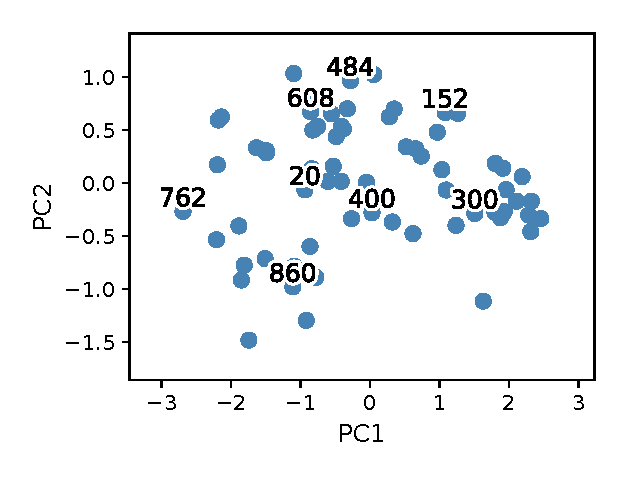
\includegraphics[width=0.6\textwidth]{../figures/fig1_pca_manifold.eps}
    \caption{\textbf{The Continuous Manifold of State Governance.} PCA projection of $N=66$ nation-states. The lack of isolated geometric clusters illustrates that regime architectures exist on a continuous spectrum.}
    \label{fig:pca_manifold}
\end{figure}

Visualizations of the institutional space (Figure \ref{fig:pca_manifold}) reveal a continuous, unbroken cloud of nation-states. There are no distinct topological chasms separating regime types; they blend seamlessly based on incremental geometric shifts. The raw three-dimensional topology (Figure \ref{fig:3d_manifold}) further corroborates this continuity. 

\begin{figure}[htbp]
    \centering
    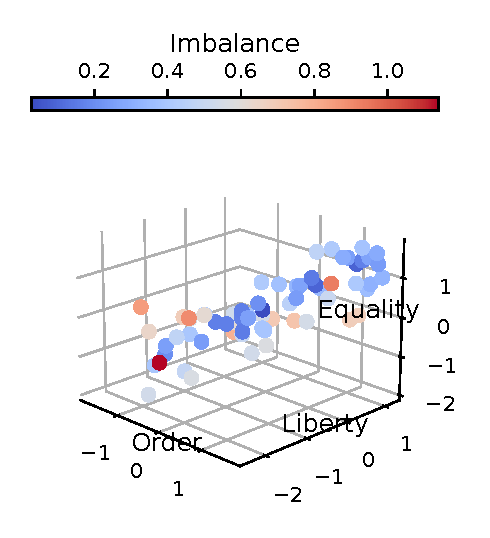
\includegraphics[width=0.5\textwidth]{../figures/fig2_3d_manifold.eps}
    \caption{\textbf{The 3D Geometry of State Governance.} A 3D scatter projection of the triad. The continuous blending visually reinforces the absence of discrete regime clusters.}
    \label{fig:3d_manifold}
\end{figure}

As a robust geometric check, a non-linear UMAP projection was applied to the triad (Figure \ref{fig:umap}). Even when allowing for non-linear manifold learning, the algorithm fails to tear the data into separate regime islands.

\begin{figure}[htbp]
    \centering
    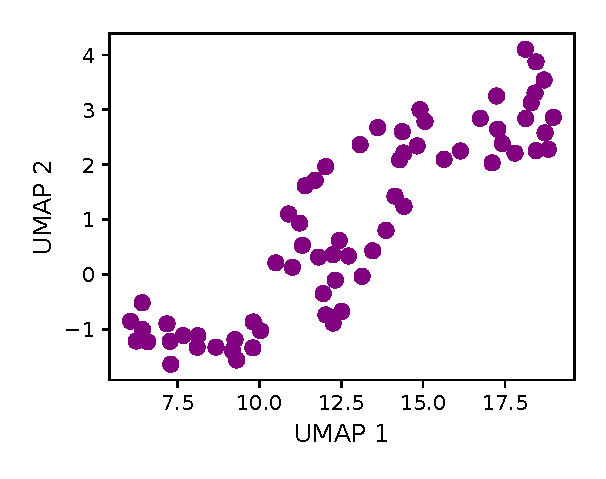
\includegraphics[width=0.6\textwidth]{../figures/fig3_umap_projection.eps}
    \caption{\textbf{UMAP Projection of State Governance.} This non-linear topological reduction confirms that nation-states form a continuous spectrum rather than isolated clusters.}
    \label{fig:umap}
\end{figure}

To test H1 formally, k-means clustering was applied. As illustrated in Figure \ref{fig:silhouette}, silhouette scores remain weak ($< 0.4$) across all values of $k$. In geometric terms, a low silhouette score indicates the absence of naturally occurring, statistically discrete clusters (Rousseeuw, 1987). This provides strong evidence consistent with H1: state governance exists on a continuous dimensional spectrum, calling into question the mathematical rigidity of discrete categorical regime typologies.

\begin{figure}[htbp]
    \centering
    \includegraphics[width=0.6\textwidth]{../figures/fig4_silhouette_scores.eps}
    \caption{\textbf{Silhouette Scores for K-Means Clustering.} Consistently low scores provide mathematical support for the continuous manifold hypothesis.}
    \label{fig:silhouette}
\end{figure}

\subsection{The Funnel of State Capacity (H2)}

Plotting Institutional Imbalance ($x$) against Magnitude ($y$) reveals a strict heteroscedastic boundary constraint, providing strong empirical support for H2. As illustrated in Figure \ref{fig:funnel}, the 10th and 90th percentile quantile regressions form an envelope that narrows dramatically as Magnitude increases. 

\begin{figure}[htbp]
    \centering
    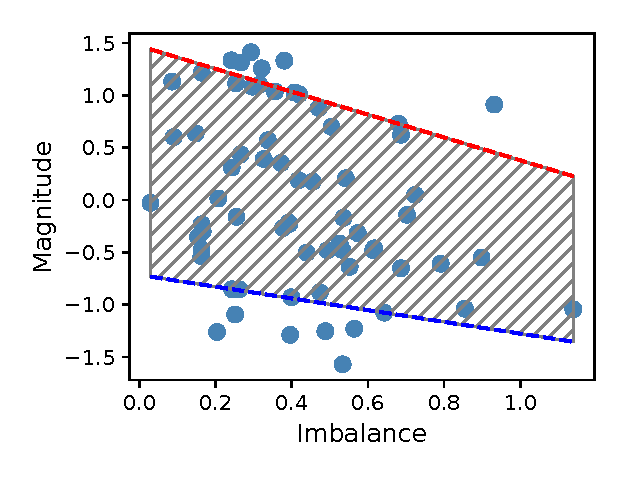
\includegraphics[width=0.6\textwidth]{../figures/fig5_funnel_capacity.eps}
    \caption{\textbf{The Boundary Constraints of State Development.} Scatter distribution of Magnitude vs. Imbalance. The dashed lines (10th and 90th percentiles) form a heteroscedastic funnel, demonstrating that achieving peak state capacity strictly requires dimensional balance.}
    \label{fig:funnel}
\end{figure}

This geometric constraint mathematically formalizes two concurrent realities of state development. First, observing the variance, the structural possibility space shrinks drastically at higher capacities: low-magnitude states can exist at almost any level of imbalance (evidenced by the wide spread at the bottom), but high-magnitude states are tightly constrained to the left side of the axis. Second, observing the upper boundary curve, the maximum achievable ceiling of Institutional Magnitude strictly decreases as Imbalance increases. It is empirically unobserved in our sample for a state to achieve the absolute highest tier of state capacity while maintaining severe structural skew. Peak governance appears to strictly require dimensional harmony.

\subsection{Outcomes and the Imbalance Premium (H3 \& H4)}

The multivariate OLS regressions provide the primary empirical test of the theoretical framework. The models exhibit strong explanatory power ($R^2 = 0.697$ for HDI and $R^2 = 0.658$ for Log GDP per capita). 

Validating H3 (Baseline Validation), Institutional Magnitude is a strong, statistically significant predictor of prosperity. A 1-unit increase in average capacity is associated with a $0.1265$ increase in HDI ($p < 0.001$) and a $0.9618$ increase in Log GDP ($p < 0.001$). 

However, testing H4 yields a profound and counter-normative discovery: the ``Imbalance Premium.'' Controlling for overall magnitude, institutional imbalance exhibits a positive, statistically significant coefficient for both HDI ($\beta = 0.1134, p = 0.005$) and Log GDP ($\beta = 1.0406, p = 0.002$). This indicates that, holding average state capacity constant, states that prioritize one axis at the expense of others actually achieve higher economic prosperity and human development than perfectly balanced states at the exact same systemic baseline.

To verify the robustness of these results, diagnostic tests were evaluated. Visual inspection of the residuals plotted against fitted values (Figure \ref{fig:residuals}) reveals a generally random distribution of errors, confirming the absence of severe heteroscedasticity. Additionally, the Durbin-Watson statistics for both models ($1.97$ and $1.82$, respectively) indicate no severe autocorrelation. While the HDI model exhibits slight non-normality in the residuals (Omnibus $p = 0.003$), the Log GDP model's residuals are highly normal (Omnibus $p = 0.874$), confirming that our standard errors and significance levels for the primary economic indicator are statistically reliable.

\begin{figure}[htbp]
    \centering
    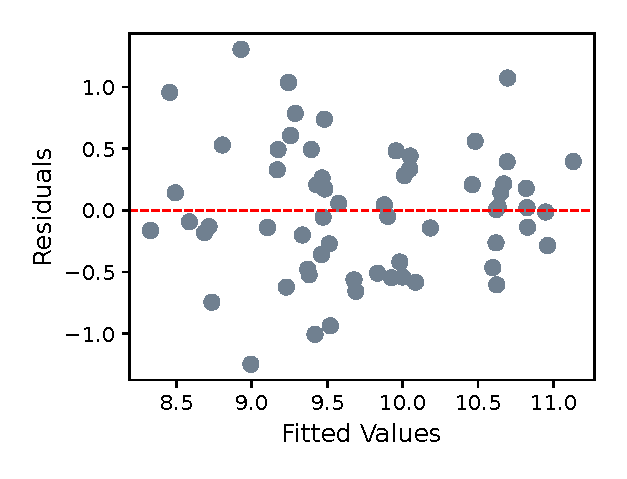
\includegraphics[width=0.6\textwidth]{../figures/fig6_residuals.eps}
    \caption{\textbf{OLS Diagnostic: Residuals vs. Fitted Values.} The random distribution of errors confirms the absence of severe heteroscedasticity.}
    \label{fig:residuals}
\end{figure}

\section{Discussion: The Vanguard Theory of Development}

\begin{figure}[htbp]
    \centering
    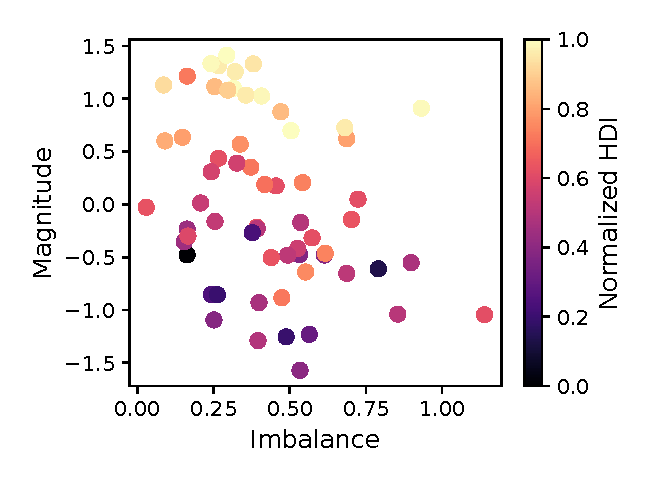
\includegraphics[width=0.65\textwidth]{../figures/fig7_hdi_map.eps}
    \caption{\textbf{The Vanguard Theory of Development.} Institutional geometries colored by normalized HDI scores. Highly imbalanced states consistently achieve higher development outcomes than balanced states at a lower capacity baseline.}
    \label{fig:hdimap}
\end{figure}

Mapping normalized HDI onto the geometric funnel (Figure \ref{fig:hdimap}) provides visual support for both the baseline effects of Magnitude (H3) and the Imbalance Premium (H4). As expected, the absolute peak of human development occurs at the top-left, confirming that maximum capacity and structural balance ultimately yield the highest societal outcomes. However, when controlling for capacity by observing the manifold horizontally, an interesting pattern emerges: at middle and lower tiers of Magnitude, heavily skewed states along the right boundary tend to achieve higher levels of development than perfectly balanced states occupying the exact same baseline capacity. While this visual trend is not universally consistent—as natural variance reveals some highly imbalanced states with comparable or slightly lower outcomes—the broader tendency aligns with the statistical premium observed in the regression models. Integrating the sequential logic of political development, we theorize two primary drivers for this geometric phenomenon:

\paragraph{1. The Authoritarian Wealth and Policy Anomaly.}
Nations prioritizing Order and Equality while systematically suppressing Liberty manifest as highly ``imbalanced'' in the manifold, yet can achieve a stable, static equilibrium of high prosperity. This often occurs in resource-rich rentier states that utilize centralized authority to drive economic extraction (Ross, 2012). Furthermore, discrete components of human development can be achieved asymmetrically via targeted policy. For instance, post-revolutionary Iran dramatically expanded women's literacy and tertiary education (Mehran, 2003)—directly boosting the nation's baseline HDI—while simultaneously restricting systemic civil liberties and political rights. This demonstrates how state capacity can artificially inflate specific developmental metrics despite profound structural skew.

\paragraph{2. The Developmental Vanguard.}
In contrast to a static anomaly, imbalance frequently serves as a dynamic, transitional phase of growth. In accordance with the principle of \textit{hierarchical concurrency}, states rarely improve Order, Liberty, and Equality symmetrically. Historical evidence suggests that breaking out of middle-income stagnation often involves a vanguard'' approach—hyper-focusing on a single institutional axis to catalyze growth. For example, the Order-first'' industrialization observed in East Asian developmental states intentionally prioritized state capacity to build the economic base required to eventually support the emergent dimensions of Liberty and broader Equality (Amsden, 1989; Wade, 1990). This pattern suggests that severe imbalance is often a functional, temporary requirement of the developmental trajectory.

\section{Conclusion}

This paper developed an axiomatic framework for the analysis of state architecture, demonstrating that political ideology and institutional design operate as a measurable geometric manifold.

The results suggest a profound paradox in political development: perfect institutional balance in the center of the manifold may represent developmental stagnation. While structural balance is ultimately required to reach the absolute mathematical limits of state capacity, dynamic economic and human development frequently requires a state to purposefully ``unbalance'' itself to break the status quo. Future research should apply longitudinal time-series data to trace the exact geometric trajectories states take as they navigate this manifold over time.

\section*{Data and Code Availability}
The Python source code, generated figures, and full replication instructions for this analysis are publicly available on GitHub at \url{https://github.com/adibatic/institutional-manifolds}. Due to licensing restrictions, the raw World Values Survey dataset is not hosted in the repository and must be downloaded separately according to the instructions provided in the repository documentation.

\section*{References}
\begin{description}

\item Acemoglu, D., \& Robinson, J. (2012). \textit{Why Nations Fail: The Origins of Power, Prosperity, and Poverty}. Crown.

\item Acemoglu, D., \& Robinson, J. (2019). \textit{The Narrow Corridor: States, Societies, and the Fate of Liberty}. Penguin.

\item Amsden, A. H. (1989). \textit{Asia's Next Giant: South Korea and Late Industrialization}. Oxford University Press.

\item Bäck, H., \& Hadenius, A. (2008). Democracy and State Capacity: Exploring a J-shaped Relationship. \textit{Governance}, 21(1), 1–24.

\item Berlin, I. (1958). \textit{Two Concepts of Liberty}. Oxford University Press.

\item Bertelsmann Stiftung. (2018). \textit{Transformation Index (BTI) Dataset}.

\item Bertalanffy, L. (1968). \textit{General System Theory: Foundations, Development, Applications}. George Braziller.

\item Blind, P. K. (2014). \textit{Policy-Driven Democratization: Geometrical Perspectives on Transparency, Accountability, and Corruption}. Palgrave.

\item Dahl, R. A. (1971). \textit{Polyarchy: Participation and Opposition}. Yale University Press.

\item Fukuyama, F. (2011). \textit{The Origins of Political Order: From Prehuman Times to the French Revolution}. Farrar, Straus and Giroux.

\item Hanson, J. K., \& Sigman, R. (2021). Leviathan's Latent Dimensions: Measuring State Capacity for Comparative Political Research. \textit{Journal of Politics}, 83(4), 1495–1510.

\item Hobbes, T. (1651). \textit{Leviathan}. Penguin Classics.

\item Huntington, S. P. (1968). \textit{Political Order in Changing Societies}. Yale University Press.

\item Liu, W., \& Li, J. (2019). Unbalanced Institutions in Market Transition: How Do They Matter for Firm Strategic Choices and Performance in Emerging Economies? \textit{Management International Review}, 59(5), 675–702.

\item Luhmann, N. (1995). \textit{Social Systems}. Stanford University Press.

\item Marshall, T. H. (1950). \textit{Citizenship and Social Class}. Cambridge University Press.

\item Mehran, G. (2003). The Paradox of Tradition and Modernity in Female Education in the Islamic Republic of Iran. \textit{Comparative Education Review}, 47(3), 269–286.

\item North, D. (1990). \textit{Institutions, Institutional Change and Economic Performance}. Cambridge University Press.

\item Rawls, J. (1971). \textit{A Theory of Justice}. Harvard University Press.

\item Ross, M. L. (2012). \textit{The Oil Curse: How Petroleum Wealth Shapes the Development of Nations}. Princeton University Press.

\item Rousseeuw, P. J. (1987). Silhouettes: A Graphical Aid to the Interpretation and Validation of Cluster Analysis. \textit{Journal of Computational and Applied Mathematics}, 20, 53–65.

\item Sen, A. (1999). \textit{Development as Freedom}. Oxford University Press.

\item Simon, H. (1962). The Architecture of Complexity. \textit{Proceedings of the American Philosophical Society}, 106(6), 467–482.

\item Transparency International. (2019). \textit{Corruption Perceptions Index Dataset}. 

\item Troyanskaya, O., Cantor, M., Sherlock, G., Brown, P., Hastie, T., Tibshirani, R., Botstein, D., \& Altman, R. B. (2001). Missing Value Estimation Methods for DNA Microarrays. \textit{Bioinformatics}, 17(6), 520–525.

\item United Nations Development Programme. (2018). \textit{Human Development Index Dataset}.

\item V-Dem Institute. (2019). \textit{Varieties of Democracy (V-Dem) Dataset}. 

\item Wade, R. (1990). \textit{Governing the Market: Economic Theory and the Role of Government in East Asian Industrialization}. Princeton University Press.

\item Wooldridge, J. M. (2015). \textit{Introductory Econometrics: A Modern Approach} (6th ed.). Cengage Learning.

\item World Bank. (2019). \textit{World Development Indicators Dataset}. 

\item World Justice Project. (2019). \textit{Rule of Law Index Dataset}. 

\item World Values Survey Association. (2020). \textit{World Values Survey Wave 7 Dataset}. 

\end{description}

\end{document}